\section{Comparación de las aproximaciones}

\subsection{Problema}

Represente en una misma gráfica los datos experimentales, la curva de ajuste por mínimos cuadrados y el aproximante de Padé del apartado a) alrededor de $t_0 = 1.5$ para los valores $\alpha$ y $\beta$ calculados en el ajuste. Calcule el error cuadrático en todos los casos y discuta la bondad de los ajustes.

\subsection{Resolución}

El código para este ejercicio se puede encontrar en \ref{code:ex5}.

Las aproximaciones se pueden ver en la siguiente figura:

\begin{figure}[H]
	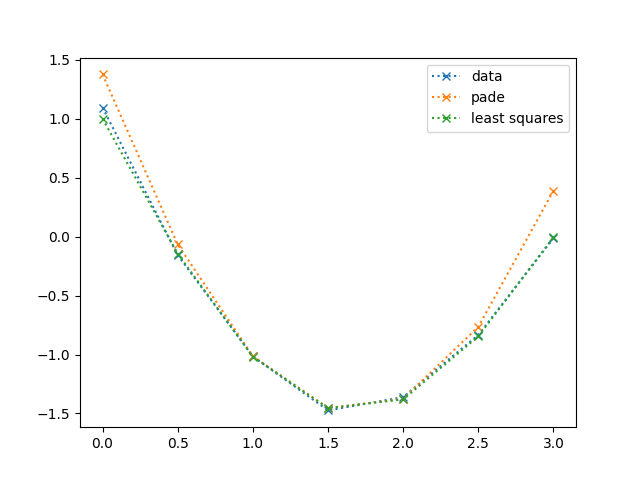
\includegraphics[width=\linewidth]{figures/compare_approx.png}
	\caption{Comparación de las aproximaciones}
	\label{fig:compare_approx}
\end{figure}

El error cuadrático, dado por:


$$
\text{SRR} = \sum_{k} (y_k - f(x_k))^2 
$$

es:
\begin{itemize}
	\item Padé: $0.254865$
	\item mínimos cuadrados: $0.010161$	
\end{itemize}

\subsection{Discusión}

Como es de esperar, la aproximación de Padé tiene mayor error que la de mínimos cuadrados, pero es aún una muy buena aproximación en la proximidad de $t_0$.

\begin{figure}[H]
	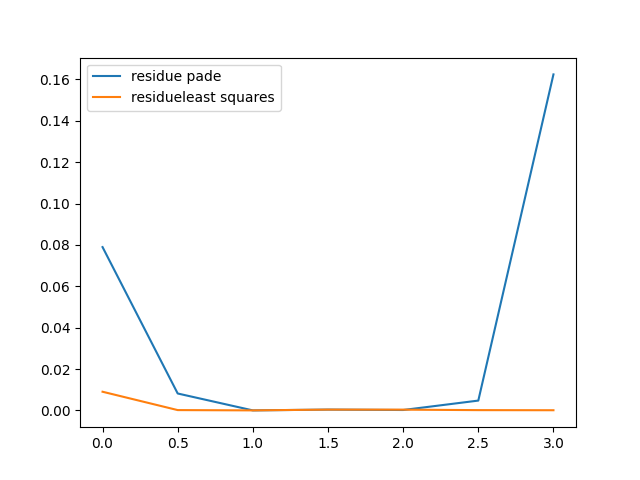
\includegraphics[width=\linewidth]{figures/errores_quad_approx.png}
	\caption{Error de las aproximaciones}
	\label{fig:error_quad_approx}
\end{figure}